% Latex Beamer template following CERN template guidelines (or trying!)

\documentclass[aspectratio=169]{beamer}
\usepackage{xcolor}
\usepackage{graphicx}
\usepackage{multicol}
\usepackage{tikz}

% Code listings with syntax highlighting
%  Require Pygments
\usepackage{minted}

\usetheme{SRR}

\newcommand{\interludeTitle}{We are here!}
\AtBeginSection[] {
    \frame{
	\frametitle{\interludeTitle}
      \begin{multicols}{2}
        \tableofcontents[
            currentsection,
            sectionstyle=show/shaded,
            ]
	  \end{multicols}
    }
}

\AtBeginSubsection[] {
	  \frame{
		\frametitle{\interludeTitle}
		\begin{multicols}{2}
        \tableofcontents[
            currentsubsection,
            subsectionstyle=show/shaded,
            ]
		\end{multicols}
	  }
}

\DeclareMathOperator*{\argmin}{arg\,min}

% Talk date
% Uncomment this to define a presentation date distinct from \today
% \def\mydate{20 Feb 2000}

% Preamble
\title[]{Voice recognition}
\subtitle{Before and after Deep Learning}
\author[]{Mikhail Kudinov}
\institute[SRR] 
{
Samsung R\&D Center Russia 
}

% Body
\begin{document}
    
    \cernSplashBlue

    % Title
    {
    \setbeamertemplate{footline}{}
    \setbeamertemplate{navigation symbols}{}
    \frame{\titlepage}
    }
    \setcounter{framenumber}{0}

    % TOC
    \frame{
        \frametitle{Table of Contents}
        \begin{multicols}{2}
            \tableofcontents
        \end{multicols}
    }



    \section{Introduction}

    \frame{
        \frametitle{This is the first slide}
        %Content goes here
        \begin{block}{Ideas}
            See how this loooks
        \end{block}
        \begin{itemize}
            \item Item 1
            \item Item 2
        \end{itemize}
    }
    
    \frame{
        \frametitle{Universal Background Model}
            \begin{columns}

                \begin{column}[t]{0.57\textwidth}
                    \begin{itemize}
                        \item Criterion: $\Lambda(X) = \log p(X|\theta_s) - \log p(X|\theta_{bck}) \geq C$
                        \item Train separate model $\theta_{bck}$ called Universal Background Model 
                        \item All frames are assumed to be independent
                        \item $p(X_t|\theta)$ is a GMM with diagonal covariance matrices $\Sigma_i$
                        \item $\theta_{bck}$ is trained with EM algorithm on the whole collection of speech data
                        \item Speaker model $\theta_{s}$ is an MAP update of $\theta_{bck}$
                    \end{itemize}
                \end{column}

                \begin{column}[t]{0.43\textwidth}
     					\begin{center}
     					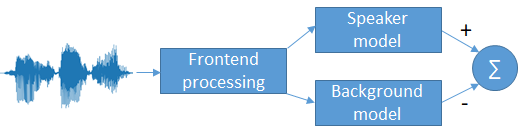
\includegraphics[width=1.0\textwidth]{images/ubm_algo.png}\\
     					\footnotesize{Likelihood ratio based system layout}
     					\end{center}               
     					\begin{center}
     					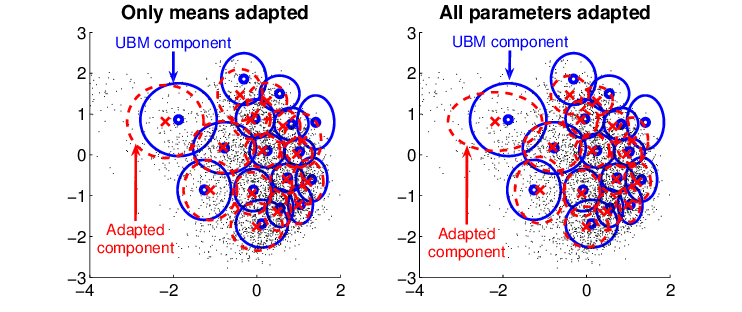
\includegraphics[width=1.0\textwidth]{images/ubm_map.png}\\
     					\footnotesize{MAP update of UBM}
     					\end{center}               				
                \end{column}
            \end{columns}
    }
    
        \frame{
        \frametitle{SVM on GMM supervectors}
            \begin{columns}

                \begin{column}[t]{0.58\textwidth}
                    \begin{itemize}
                        \item Supervector $m$: do MAP-updates of means of the UBM and concatenate them
                        \item Use lower-bound on KL-divergence as a distance measure:
%                        \[
%                            \mathbb{D}(p(x)||q(x)) \leq \sum_i \pi_i \mathbb{D}(\mathcal{N}(\mu^p_i, \Sigma_i)||\mathcal{N}(\mu^q_i, \Sigma_i))
%                        \]
                        $d(m^a, m^b) = \frac{1}{2} \sum_i \pi_i (m^a_i - m^b_i)\Sigma^{-1}_i(m^a_i - m^b_i)$
                        \item Use SVM on supervectors with the kernel defined above
                        \item Nuisance attribute projection
                    \end{itemize}
                \end{column}

                \begin{column}[t]{0.42\textwidth}
     					\begin{center}
     					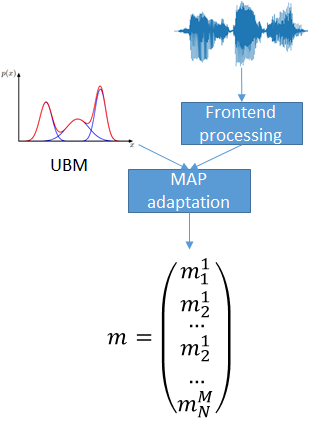
\includegraphics[width=0.6\textwidth]{images/svm-sv.png}\\
     					\footnotesize{Supervector computation}
     					\end{center}                             				
                \end{column}
            \end{columns}
    }
    
        \frame{
        \frametitle{Extensions of supervector model}
  %          \begin{columns}
              %  \begin{column}[t]{0.58\textwidth}
                    \begin{itemize}
                        \item SVM with simple cosine kernel on preprocessed supervectors
                        \item Within-class Covariance Normalization
                        $k(m_1, m_2) = m_1W^{-1}m_2,$\\
                        where $W$ is a covariance matrix:
                        $W = \frac{1}{S}\sum_{s=1}^S \frac{1}{n_s}\sum_{i=1}^{n_s}(m_i^s - \overline{m_s})(m_i^s - \overline{m_s})^t$
                        \item SVM on LDA-projected supervectors
                        \item Nuisance Attribute Projection
                        $\argmin_P \sum_{i,j} W_{i,j}\|Pm_1 - Pm_2\|_2^2$, where $W_{i,j} = 0$ iff $w1$ and $w2$ are from e.g. different microphones (nuisance channel direction)
						\item Joint Factor Analysis
                        \item Probabilistic LDA (PLDA)
                    \end{itemize}
     				                           				
      %          \end{column}
  %          \end{columns}
    }
    
            \frame{
        \frametitle{Joint Factor Analysis in Speaker Verification}
  %          \begin{columns}
              %  \begin{column}[t]{0.58\textwidth}
                    \begin{itemize}
                        \item Joint Factor Analysis: $m = \mu + Vy + Ux + Dz$, where $y$ is a speaker-dependent and $x$ is a channel-dependent vector
                    \end{itemize}
     				                           				
      %          \end{column}
  %          \end{columns}
    }
    
    \frame{
        \frametitle{i-vectors}
          \begin{itemize}
           \item Front-end Factor Analysis for a supervector $M$:
                        $m = \mu + Tw$, where $\mu$ is the speaker- and channel-independent vector (UBM-vector)
           \item $T$ is a rectangular matrix of low rank 
           \item $w \sim \mathcal{N}(0, \mathbb{I})$ is called \textit{i-vector}
           \item i-vector estimation for known matrix $T$ for utterance $u$:
           \item[]
           \begin{itemize}
             \item Use UBM $\Omega$ to get Viterbi or Baum-Welch estimations for GMM component $c$: 
             $N_c=\sum_{t} P(c|y_t, \Omega)$;
            $F_c=\sum_{t} P(c|y_t, \Omega)(y_t-\mu_c)$
            \item $w = (I + T^T\Sigma^{-1}NT)^{-1}T^T\Sigma^{-1}F$, where $N$ and $F$ are concatenations of $N_c$ and $F_c$ for all GMM components $\lbrace c_i \rbrace$
           \end{itemize}
           \item $T$ is estimated using ML algorithm
           \end{itemize}
    }
    
        \frame{
        \frametitle{DNNs for better i-vector extraction}
          \begin{columns}
             \begin{column}[t]{0.58\textwidth}
                \begin{itemize}
                   \item Use DNN to obtain class-posterior for statistics collection $N$ and $F$ for i-vector calculation
                   \item Classes are context-aware \textit{senones}
                   \item Requires ASR system trained separately
                   \item Similarity score is computed on PLDA-projections
                \end{itemize}
             \end{column}
           \begin{column}[t]{0.42\textwidth}
                \begin{center}
     			    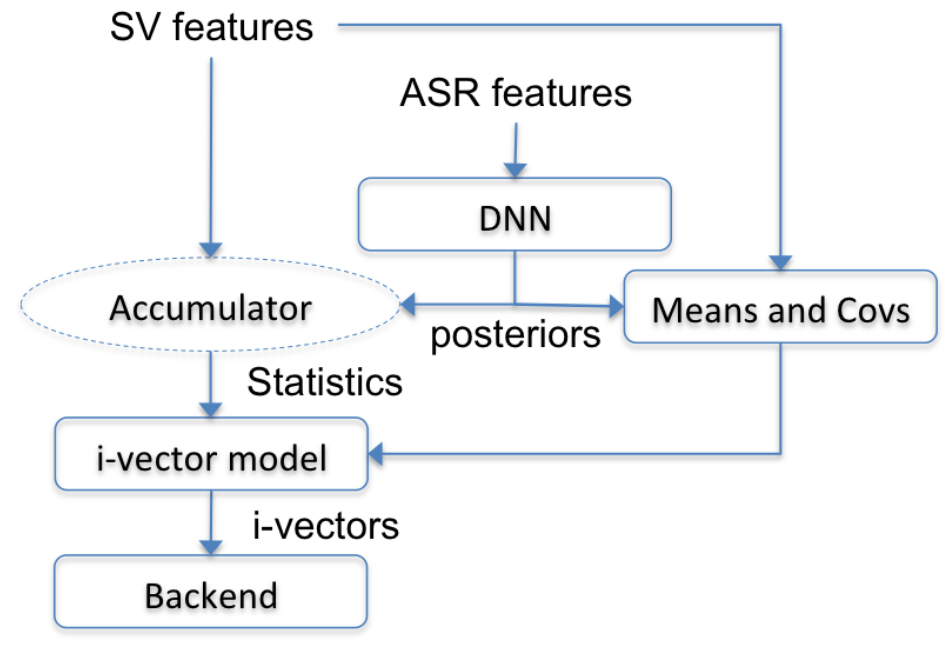
\includegraphics[width=0.9\textwidth]{images/dnn-i-vector.png}\\
     				\footnotesize{DNN/i-vector framework}
     		    \end{center}
           \end{column}
          \end{columns}
    }
    
     \frame{
        \frametitle{GMM-UBM on bottleneck features}
          \begin{columns}
             \begin{column}[t]{0.58\textwidth}
                \begin{itemize}
                   \item Use DNN predicting senone classes to train a bottleneck mapping
                   \item Use first layers of the DNN as a bottleneck features extractor
                   \item Train traditional GMM-UBM/i-vector system on the bottleneck features
                \end{itemize}
             \end{column}
           \begin{column}[t]{0.42\textwidth}
                \begin{center}
     			    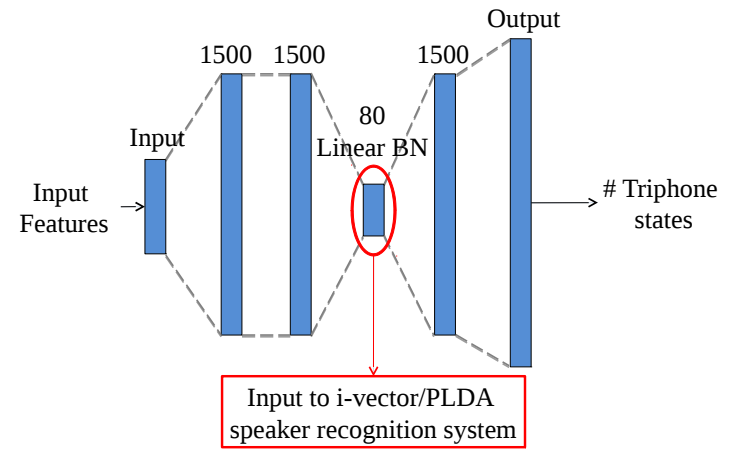
\includegraphics[width=0.9\textwidth]{images/bottleneck.png}\\
     				\footnotesize{DNN for bottleneck features extraction}
     		    \end{center}
           \end{column}
          \end{columns}
    }
    
         \frame{
        \frametitle{d-vectors}
          \begin{columns}
             \begin{column}[t]{0.58\textwidth}
                \begin{itemize}
                   \item Train a DNN to predict speaker label by a short speech segment
                   \item Use last hidden layer as a feature vector
                   \item At the enrollment stage average of last hidden layers for each speech frame is used as a speaker vector
                   \item At the identification stage the decision is made according to a particular distance metric
                \end{itemize}
             \end{column}
           \begin{column}[t]{0.42\textwidth}
                \begin{center}
     			    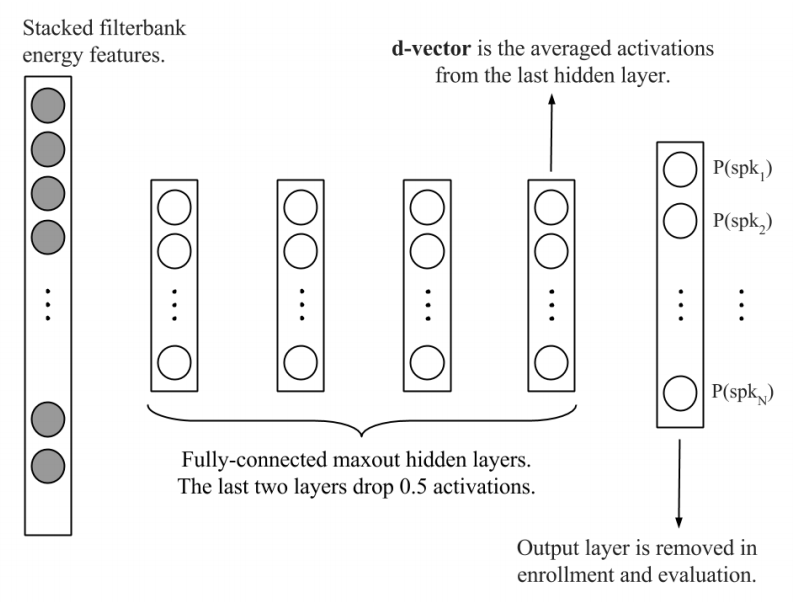
\includegraphics[width=0.9\textwidth]{images/d-vector.png}\\
     				\footnotesize{DNN for d-vector extraction}
     		    \end{center}
           \end{column}
          \end{columns}
    }
    
        \frame{
        \frametitle{Text-independent end-to-end Speaker verification/x-vectors}
          \begin{columns}
             \begin{column}[t]{0.5\textwidth}
                \begin{itemize}
                   \item Add global average pooling to handle problem of different lengths
                   \item Use objective similar to metric learning
                   \[
                   P(x,y) = \frac{1}{1+e^{-L(x,y)}}
                   \]
                   \[
                   L(x,y) = x^Ty - xSx - ySy + b
                   \]
                   \begin{equation*}
                   \begin{split}
                   E = & -\sum_{(x,y) \in Same} \log P(x,y) \\ &- K\sum_{(x,y) \not \in Same} \log (1 - P(x,y))
                   \end{split}    
                   \end{equation*}
                \end{itemize}
             \end{column}
           \begin{column}[t]{0.5\textwidth}
                \begin{center}
     			    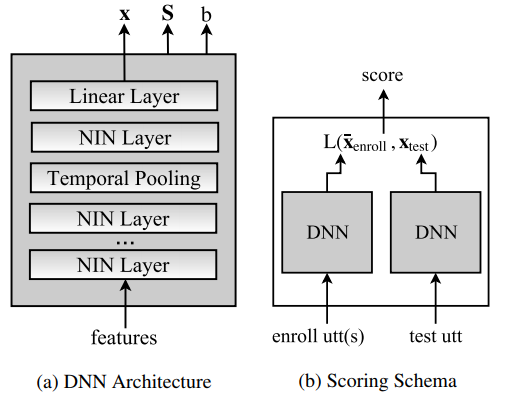
\includegraphics[width=0.8\textwidth]{images/end2end.png}\\
     				\footnotesize{DNN scoring}
     		    \end{center}
           \end{column}
          \end{columns}
    }


	% This block includes a picture full slide
	{ % all template changes are local to this group.
		\setbeamertemplate{navigation symbols}{}
		\begin{frame}[plain]
			\begin{tikzpicture}[remember picture,overlay]
			\node[at=(current page.center)] {
				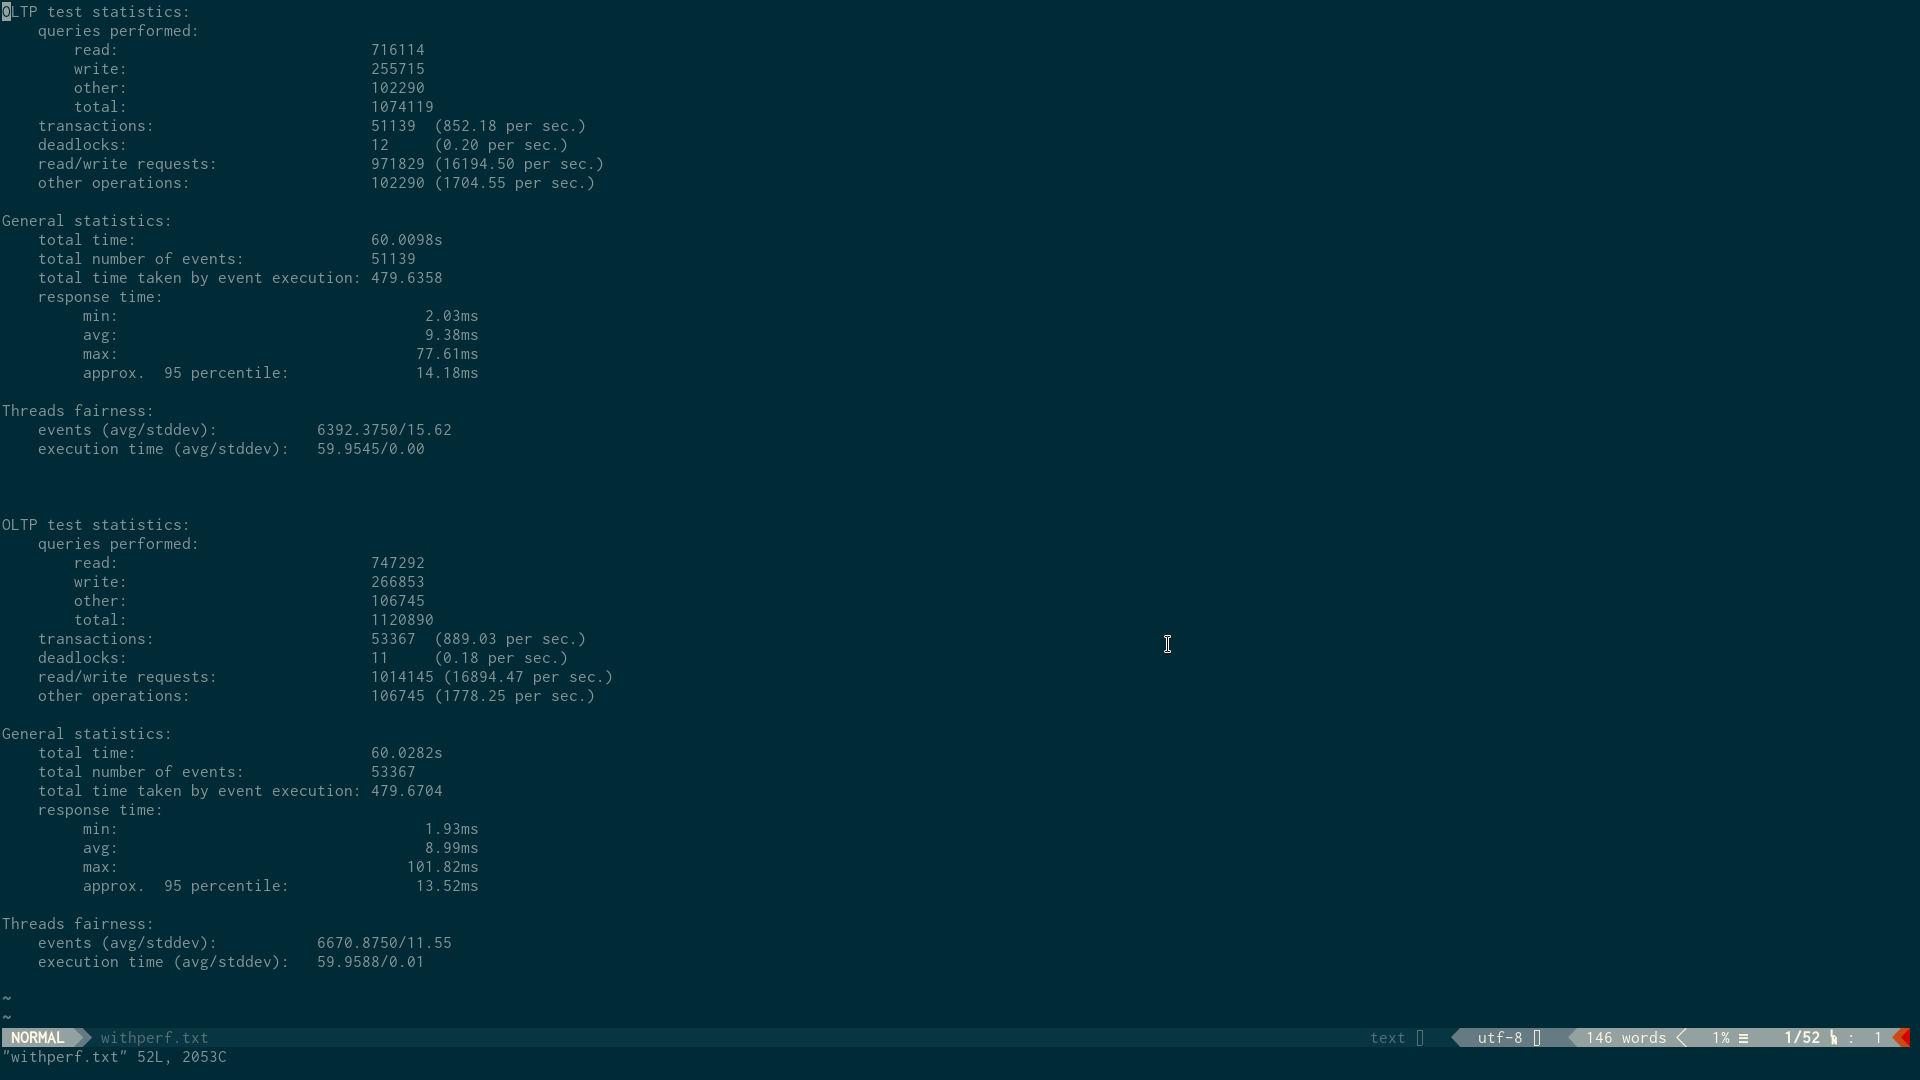
\includegraphics[width=\paperwidth]{images/image.png}
			};
			\end{tikzpicture}
		\end{frame}
	}

    % This slide has code block with syntax highlighting using the Minted package
    %  Minted requires Pygments and building the PDF with the --shell-escape argument
    %  for pdflatex
    \begin{frame}[fragile]
        \frametitle{This slide has code blocks}
		\begin{minted}[
			frame=lines,
			framesep=2mm,
			baselinestretch=1.2,
			fontsize=\footnotesize,
			linenos
			]{python}
        import numpy as np
         
        def incmatrix(genl1,genl2):
            m = len(genl1)
            n = len(genl2)
            M = None #to become the incidence matrix
            VT = np.zeros((n*m,1), int)  #dummy variable
        \end{minted}
\end{frame}


    \subsection{Intro subsection}
    \frame{
        \frametitle{This is the second slide}
        \framesubtitle{A bit more information about this}
        %More content goes here
        \begin{alertblock}{Alert block}
            Alert text
        \end{alertblock}
    }
    
    \section{Section 1}

    \frame{
        \frametitle{Generic slide}
        \framesubtitle{A bit more information about this}
        %More content goes here
    }
    \section{Section 2}

    \frame{
        \frametitle{Generic slide}
        \framesubtitle{A bit more information about this}
        %More content goes here
    }

    
    \section{Conclusion}
    
    \frame{
        \frametitle{Generic slide}
        \framesubtitle{A bit more information about this}
        %More content goes here
    }
    
    \section{Acknowledgements}
    
    \frame{
        \frametitle{Generic slide}
        \framesubtitle{A bit more information about this}
        %More content goes here
    }

    \section{}
   % \cernSplashWhite

\end{document}

